\frame
{
	\frametitle{Fichier DICOM}
	\begin{itemize}
		\item Single Frame
		\begin{itemize}
			\item Une image: stock\'ee dans un fichier.
			\item Une coupe = une image
		
			$\Rightarrow$ s\'erie de 100 coupes = 100 fichiers.
		\end{itemize}
		\item<2-> Multiframe
		\begin{itemize}
			\item Aussi appel\'e \emph{Enhanced DICOM}.
			\item Plusieurs images dans la m\^eme s\'equence.
			
			E.g. s\'equence vid\'eo d'\'echographie.
		\end{itemize}
		\item<3-> Arborescence des r\'epertoires/fichiers
		\begin{center}
			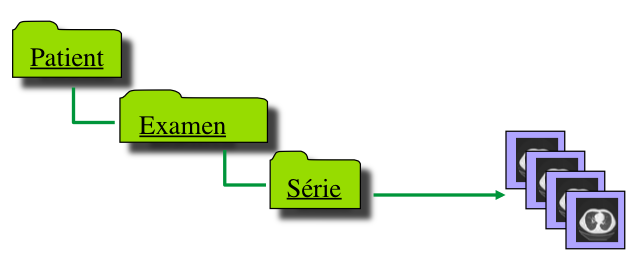
\includegraphics[width=.8\linewidth]{../figures/arborescence.png}
		\end{center}

	\end{itemize}
}

\frame
{
	\frametitle{Contenu d'un fichier {.dcm}}
	
	Un fichier DICOM est l'agr\'egation des \'el\'ements suivants:
	\begin{itemize}
		\item<2-> Pr\'e-ent\^ete:
		\begin{itemize}
			\item<2-> Pr\'eambule: 128 octets de donn\'ees \emph{application}.
			\item<2-> Pr\'efixe: 0x4449434D=DICM (4 octets).
		\end{itemize}
		\item<3-> Suite de Data Elements:
		\begin{itemize}
			\item<4-> Tag;
			\item<5-> VR;
			\item<6-> Taille;
			\item<7-> et Valeur (qui peut \^etre une s\'equence).
		\end{itemize}
		\item<8-> Et l'image, un Data Element.
	\end{itemize}
}


\frame
{
	\frametitle{Exemple en pratique}
	Exemples avec OsiriX et Weasis.
}
